\subsubsection{Play Piano}
Sơ đồ use-case Play Piano:
\begin{figure}[H]
    \centering
    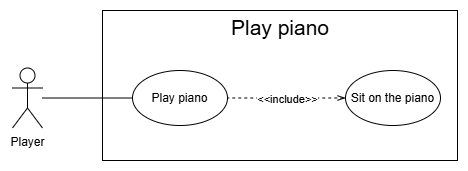
\includegraphics[width=0.75\linewidth]{4.Đặc tả chi tiết các lược đồ/Use-case/images/PlayPiano.png}
    \caption{Use-case mô tả Play Piano}
    \label{fig:placeholder}
\end{figure}


\begin{table}[H]
\centering
\begin{tabular}{|p{4cm}|p{10cm}|}
\hline
\textbf{Use-case name} & Play Piano \\ \hline
\textbf{Actor} & Người chơi \\ \hline
\textbf{Descriptions} & Use-case này sẽ chỉ ra các bước cần thực hiện để có thể chơi đàn piano. \\ \hline
\textbf{Pre-conditions} & Phải vào được trong lobby \\ \hline
\textbf{Trigger} & Không có. \\ \hline
\textbf{Post-conditions} & Không có \\ \hline
\textbf{Normal Flow} &
\begin{enumerate}
\item Người chơi di chuyển đến trước ghế ở piano.
\item Người chơi nhấn giữ \textbf{''F''} để ngồi vào ghế.
\item Người chơi bắt đầu chơi đàn bằng cách nhấn 7 phím đầu tiên của 3 hàng trên bàn phím.
\item Người chơi nhấn giữ \textbf{''F''} để đứng dậy.
\item Use-case kết thúc sau khi người chơi đứng dậy.
\end{enumerate}
\\ \hline
\textbf{Alternative Flow} &
Không có
\\ \hline
\textbf{Exception Flow} &
Không có
\\ \hline
\end{tabular}
\end{table}